
模型的建立需要平衡真实性、预测性和普适性\cite{gunderson2017}。
流域系统模型旨在描述水的地球物理过程动力学及人类管理元素(如基础设施、机构和治理)\cite{hadjimichael2020}。
流域人水系统包括空间尺度依赖的地表生态过程、系统层次变量反馈的动力过程和多尺度的复杂人水相互作用\cite{bodin2017b,sayles2017,sayles2019}。
因此,流域人水系统的建模方法主要包括:基于传统分布式水文模型耦合人类活动模块发展而来的分布式社会-水文模型(图\ref{ch1:fig:models}~A);在系统或区域层次上耦合来自社会的系统动力学模型,用于模拟生态系统关键变量(图\ref{ch1:fig:models}~B);以及自下而上对流域内复杂人-水互动进行仿真的多主体模型(图\ref{ch1:fig:models}~C)。

\begin{figure}[!h]
    \centering
    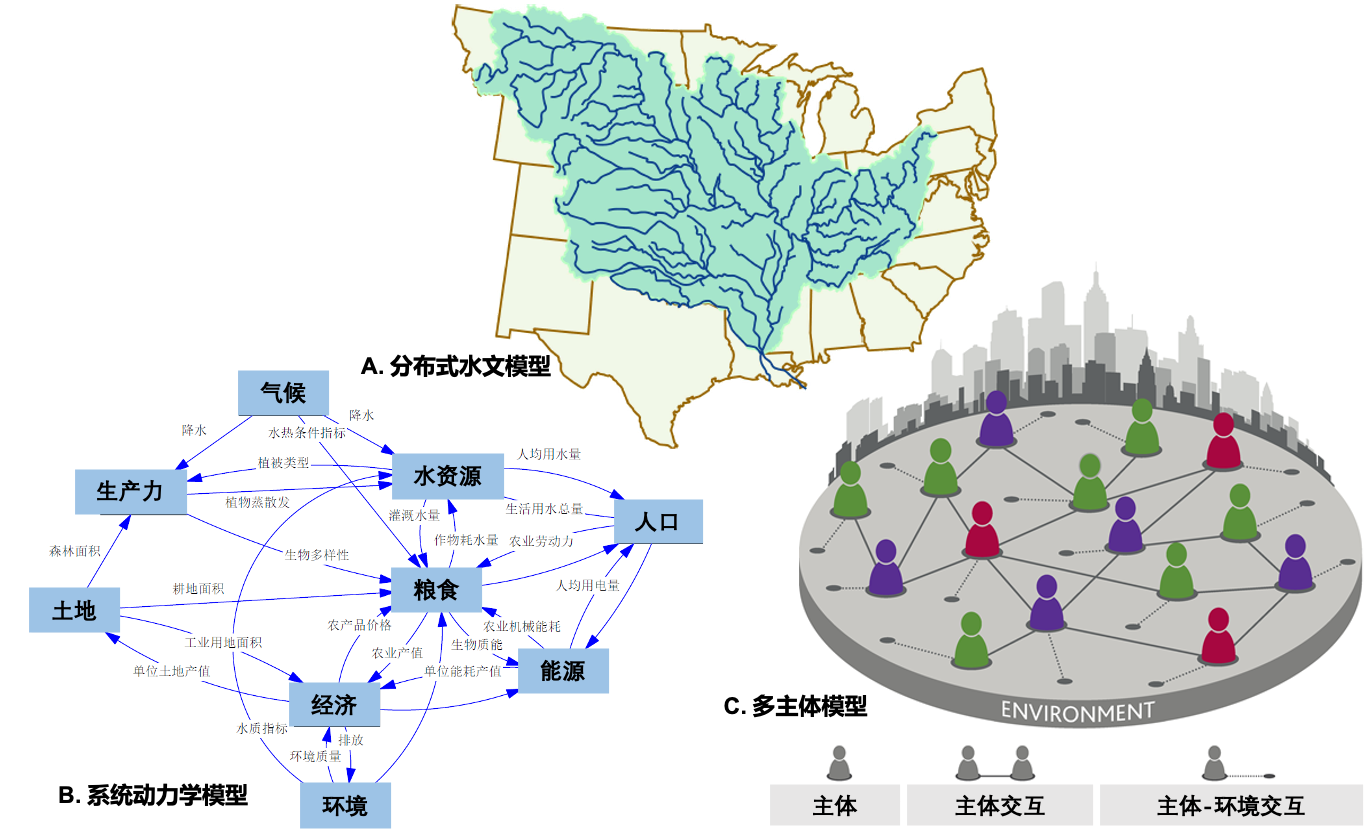
\includegraphics[width=\textwidth]{img/ch1/ch1_models.png}
    \caption[流域人水系统的建模方法示意图]{流域人水系统的建模方法示意图。}\label{ch1:fig:models}
\end{figure}

\subsubsection{分布式社会-水文模型}

分布式流域水文模型相对于传统的集总式水文模型,充分考虑了流域内水文过程的异质性\cite{wangzhonggen2003},是目前流域研究的主流工具。
常见的分布式水文模型有SWAT模型、新安江模型、陕北模型、布式时变增益水循环模型等,这些模型在国内外得到了广泛的应用\cite{arnold1998,xiajun2003,ficklin2009}。
流域分布式模型通过耦合生态过程,还可以描述大尺度流域陆地生态演变过程,如国外的SWIM模型\cite{krysanova2005}、RHESSys模型\cite{tague2004}、Budyko–Choudhury–Porporato模型\cite{donohue2012}等都属于这类生态-水文模型。

现有的分布式水文模型由于构建原理及最初率定区域的不同,导致模型侧重点有所不同。例如,SWAT模型侧重描述产流过程\cite{wangzhonggen2003a},而LISTFLOOD模型则侧重于模拟水动力过程、洪水过程等\cite{zengzhaoyang2017}。
然而,现有的分布式模型仍较少将人为干预水文过程的因素作为模拟重点。
贾仰文等人开发的WEP-L分布式流域二元水循环模型是具有物理机制的流域分布式水循环模型,考虑了人类取用水和水利水保工程等因素对水循环过程的影响,实现了“自然-社会二元水循环”过程的耦合模拟和分析\cite{jia2010}。
2019年,国际应用系统分析研究所(International Institute for Applied Systems Analysis, IIASA)开发了基于社区的水文模型(Community Water Model, CWatM)模型,将水库调度等水资源管理要素也纳入了模型\cite{burek2020}。
但迄今为止,仍然缺乏将水资源治理制度(如法律法规)等人类活动要素的影响作为流域分布式模型模拟的重点的研究。

\subsubsection{自上而下的系统动力学模型}

% 江本子
系统动力学模型能够从整体层面解析系统要素之间的关联、反馈和演化过程\cite{jaeger2017},并预测关键变量和反馈机制在变化环境下的变化\cite{vaighan2017}。
目前许多大尺度评估模型都采用了系统动力学模型,如ANEMI3和T21 China模型,这些模型都包含了自然和社会系统的多个部门,并反映了它们之间的相互作用\cite{breach2021, qu2020}。
因此,流域人水系统的系统动力学模型可以通过分析系统间的相互作用、内部结构变化等现象,揭示流域人-水关系的动态特征。
将研究范围限制在流域尺度的系统动力学模型考虑流域特征时,可使模拟结果更符合实际情况。
例如,ANEMI Yangtze是在ANEMI3基础上针对长江流域建立的系统动力学模型\cite{jiang2022},将长江的渔业作为模型的外生变量考虑进去,能够分析十年禁渔政策对流域系统的影响\cite{jiang2022}。

人类活动作为系统内部反馈循环的关键变量,也可以被纳入系统动力学模型进行考虑。
Viglione 和 Baldassarre 等人在流域尺度构建了用于解释和预测人类社会与洪水互相反馈、协同演化的系统动力学模型\cite{viglione2014,dibaldassarre2015},其中水文要素(洪水)和社会组分(例如公众意识、风险文化、经济发展等)被视为反馈过程的核心变量\cite{song2021a,ciullo2017}。
Muneepeerakul 等人则提出了一个流域社会-生态系统的发展轨迹模型,以探讨什么情况下稳定的治理结构可以促使堤坝等公共基础设施在系统中内生地出现\cite{muneepeerakul2017}。
系统动力学模型的劣势包括缺乏对流域系统空间特征的识别,这在流域研究中非常重要。
系统动力学模型还需要通过基于数据或经验的函数自上而下地建立系统要素间关系的假设,对于较为复杂且尚缺乏充分研究的流域系统变化,建模将面临很大的困难。

\subsubsection{自下而上的多主体模型}

自下而上的多主体模型(Agent-based model)能够将不同利益相关者,如管理者、水用户等,作为系统的不同主体进行考虑,研究他们的相互影响关系,以研究流域人水系统层面的涌现\cite{biggs2021}。
自组织(Self-organization)是指一种从初始无序系统的局部相互作用中,产生某种形式整体秩序的过程\cite{berkes2008},系统所有组成部分本身没有的属性可能因此而涌现(Emergence)。
人-水系统作为开放的复杂系统,涌现的宏观演化属性是各种广泛存在的相互作用的结果\cite{schluter2019}。
Manson等人研究了在制度、社会网络和其他农户行为的影响下,土地利用格局的涌现\cite{manson2016}。
Castilla-Rho等人利用多主体建模应用于地下水资源管理,发现社会规范的参数能够解释地下水资源可持续治理模式的涌现\cite{castilla-rho2017a,castilla-rho2015,castilla-rho2019,castilla-rho2017}。

过去,受限于验证困难和计算量大的特性,多主体模型常常使用简单机制模型探索系统层面的涌现与发展轨迹,对于复杂环境条件的刻画并不够准确\cite{biggs2021}。
然而,近年来随着计算机算力提升和各类仿真算法的增强,越来越多的多主体模型开始尝试结合带有空间分布的实际数据进行建模,仿真复杂多变的社会-生态系统\cite{steger2021}。
Grêt-Regamey等人通过结合调查统计数据,使用多主体模型证明了行为者多样性对提高社会-生态系统对全球变化的弹性的重要作用\cite{gret-regamey2019}。
Cuthbert等人则借助非洲早期的水资源分布数据,证明了“逐水而居”可能是人类早期迁徙演化的重要驱动力\cite{cuthbert2017}。
Sayles等人结合多主体模型与网络分析,研究了流域尺度社会-生态的制度匹配,证明了制度与生态连接脆弱的区域容易产生生态问题\cite{sayles2017}。

综上所述,建模已成为研究人-水系统演变机制的重要手段。
然而,目前比较成熟的分布式水文模型严重忽略了政策制度等非工程人为因素,系统动力学模型则缺乏重要的空间信息。
自下而上的多主体模型能够仿真流域内部复杂的人-水关系,随着计算机算力的提升,其结合复杂环境空间分布数据的能力正不断增强,是揭示流域系统层面人-水关系变化机制的理想建模方法。
